\chapter{Naive Solution}
\label{chap:naivesoln}

To compare the efficiency of our approach, we present a straightforward solution for processing Spatial Alarms in Obstucted Space. 
In Section~\ref{naiveview}, we give an overview of the naive solution. Section~\ref{naivealgo} presents the algorithm of the solution.

\vspace*{12pt}

\section{Overview}
\label{naiveview}
In a spatial alarm query a user provides a POI type and a distance and the query triggers the alarm. The naive approach to evaluate spatial alarm is a simple approach which works in the following steps:
\begin{itemize}
\item User's location and alarm range are sent to the server.
\item Server constructs the visibility graph using the POIs and obstacles within radius $r$ of user
\item Server returns the visibility graph to the client.
\item Client computes the obstructed distance of POIs in range $r$.
\item If any alarm's obstructed distance is less than $r$, then an alarm is triggered.
\item As soon as the client moves again, the whole process is repeated.
\end{itemize} 
This approach searches for a new alarm in the known region as soon as the client changes it's position.


\vspace*{12pt}

\section{Algorithm}
\label{naivealgo}
The input to the Algorithm \ref{GetAlarmables} is the location of the client $q$ and the search radius $r$. The Output of the Algorithm is the visibility graph $V_G$.
In the Algorithm \ref{GetAlarmables}, the \textsc{GetAllPOI}($q, r$) function populates the set $P$ of POIs within the radius $r$ centring the query point (the client's current location) $q$. Similarly, \textsc{GetObstacleSet}($q, r$) function returns the set of all obstacles within the radius $r$ centring $q$.\\

\textsc{MakeVisGraph}$(P,O)$ function returns the \textit{visibility graph} $V_G$ with the set of POIs $P$ and the set of obstacles $O$.

Here, a \textbf{Visibility Graph} \cite{VG1},\cite{VG2},\cite{VG3},\cite{VG4} is a graph $V_G(V,E)$ where each $v \in V$ is either a POI or a data-point and for each $(u,v) \in E$, there is an edge $e$ between $u$ and $v$ if and only if it does not intersect with any obstacles $i.e.$ $u$ and $v$ are \textit{visible} to each other along the edge $e$.\\

\begin{figure}[h]
  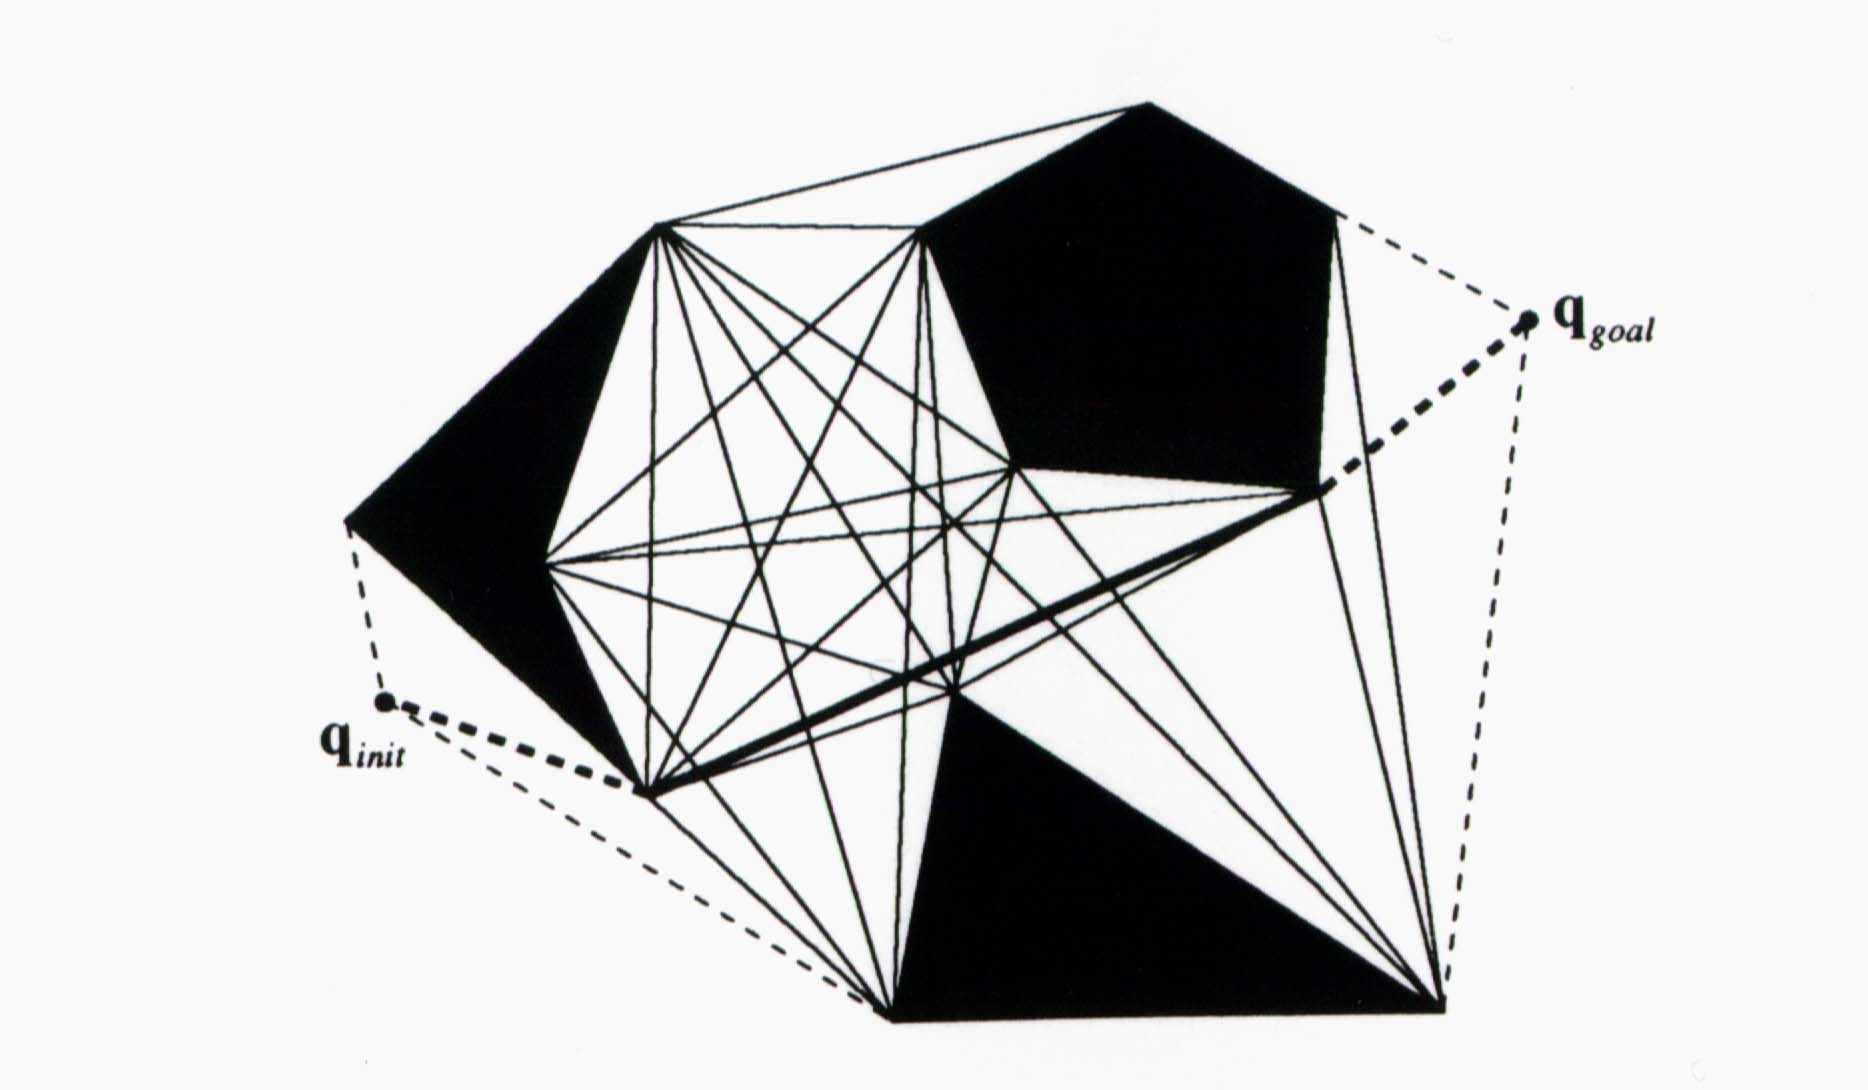
\includegraphics[width=\linewidth]{visibility_graph.jpg}
  \caption{Visibility Graph}
  \label{fig:visgraph}
\end{figure}
\vspace{5pt}
$\textsc{MakeAnswerSet}(q, V_G)$ function returns a heterogeneous data-model consisting of its all parameters to be used by the caller client-side program.


\DontPrintSemicolon
\begin{algorithm}
\caption{\textsc{GetAlarmables}($q$, $r$ , $A_{prev}$)}
    \SetKwInOut{Input}{Input}
    \SetKwInOut{Output}{Output}
    \Input{Query point $q$ and the search radius $r$}
    \Output{The visibility graph $V_G$} 
	
	 $P \gets \textsc{GetAllPOI}(q, r)$ \;
	 $O \gets \textsc{GetObstacleSet}(q, r)$ \;
	 $V_G \gets \textsc{MakeIncrementalVisGraph}(P, O, A_{prev},V_g)$ \;
	 $D_O \gets \textsc{getAllObstructedDist}( q, V_g )$
	\Return \textsc{MakeAnswerSet}$(q, V_G,D_O)$ \;
\label{GetAlarmables}
\end{algorithm}

The following method is triggered on any change of the user's location by the system checking whether to give any alarm to the client or not along with the check of necessity to fetch more POI and obstacle when the client goes outside of the farthest POI's alarming zone.
Here, the function \textsc{AlarmUser}$(p_i)$ triggers an alarm to the user since the respective POI $p_i$ is reached and also marks $p_i$ to be reached in the set of POIs $P$. \\
The inputs to the Algorithm \ref{UpdateClient} are the current client-location $q$ and the answer set $A$ consisting of the region's center $q$,% minimum distance to be covered by the client to trigger this update procedure $k{min}$,%
POI set $P$, obstacle set $O$, and the visibility graph $V_G$.
\begin{algorithm}
\caption{\textsc{UpdateClient}$(q, A)$}

    \SetKwInOut{Input}{Input}
    \SetKwInOut{Output}{Output}
    \Input{Client's current location $q$, latest answer set $A$}
    
	 \ForEach{$p_i \in P$} {
		\If{$dist_O(q, p_i, V_G) > p_i.u$}{
			$\textsc{AlarmUser}(p_i)$\;
		}
	}
	 \If {$dist_E(A.q, q) > A.d_u$ }{
		\textsc{GetAlarmables}$(q, 100)$
	}
\label{UpdateClient}
%\end{algorithmic}
\end{algorithm}


%The run-time of the first line of the second procedure \ref{UpdateNaive1} is $O(\left\vert{P}\right\vert)$, whereas the second line depends on the amount of location-change and the FetchPOI procedure.
In this naive-approach, the visibility-graph is constructed more times than necessary to hold accuracy, each of which constructions requires $O(n^2)$ \cite{mur}, where $n =$ the number of edges of the obstacles. A huge overhead is also sufficed to make $P$ and $O$ sets using such procedure. Again, the Algorithm \ref{GetAlarmables} can also be run much less time than in this approach, which is improvised in the later approach.





